\section{Methoden zur Klassifizierung von OCT Aufnahmen der Retina}
\subsection{Tiefes faltendes neuronales Netz (CNN)}
Die Klassifizierung von OCT Aufnahmen der Retina stellt eine Aufgabe der Bildklassifizierung dar. Für die Bildklassifizierung durch maschinelles Lernen haben sich in der Praxis tiefe faltende neuronale Netze (CNN) bewährt. Das bekannteste Beispiel stellt das Erkennen von handgeschriebenen Zahlen dar, wobei eine nahezu menschliche Genauigkeit erreicht werden kann \cite{MNIST}. Daher wird auch im Rahmen dieser Projektarbeit auf diesen Typ der tiefen neuronalen Netze zurückgegriffen. \\
Die Aufnahmen des verwendeten Datensatzes besitzen unterschiedliche Dimensionen und werden vor der Übergabe an das CNN auf eine einheitlich Größe von $(400\times 400)$ skaliert. Pixel, die bei diesem Vorgang zu der Aufnahme hinzugefügt werden, werden weiß eingefärbt. Zudem werden die alle Pixelwerte des Datensatzes auf den Wertebereich $[0,\,1]$ linear transformiert. \\ 
Demzufolge erhält das CNN die Pixelwerte in Form einer zweidimensionalen Liste der Dimension $(400\times 400)$ als Eingangswerte. Ein CNN besteht in der Regel hauptsächlich aus drei Bestandteilen, den sogenannten faltenden Lagen, welche im Folgenden als Conv2D Lagen bezeichnet werden, den Aggregationsschichten, die mehrere Neuronen einer Conv2D Lage zu einem Neuron zusammenfassen und welche im Folgenden als Pooling Lagen bezeichnet werden, und flache vollständig vernetzte dichte Lagen. In den faltenden Lagen wird die Dimension einer Faltungsmatrix (Kernel) definiert, welche die zweidimensionale Neuronenstruktur in festgelegten Schrittweiten abrastert. Bei jedem Schritt wird über eine diskrete Faltung die Aktivität jedes Neurons, die innerhalb des Kernels liegen, berechnet. Die Addition der Aktivitäten der einzelnen Neuronen ergibt den Ausgangswert für jeden Schritt. Anschaulich bedeutet dies, dass eine $(400\times 400)$ Neuronenstruktur, die beispielsweise mit einem $(2 \times 2)$ Kernel in Schrittweiten der Form $(2,\,2)$ abgerastert wird, eine Ausgangsstruktur der Form $(200\times 200)$ generiert. Die Anzahl der Kernel, die zur Abrasterung benutzt werden, wird ebenfalls in jeder Conv2D Lage festgelegt.  \\
Für die Pooling Lage wird die Dimension eines Fensters festgelegt, welches die Probe abfährt und bei jedem Schritt die Neuronen innerhalb dieses Fensters zu einem Neuron zusammenfasst. Wird beispielsweise ein $(2\times 2)$ Fenster definiert, welches eine $(200 \times 200)$ Neuronenstruktur ohne Überlappung der einzelnen Schritte abfährt, werden in jedem Schritt vier Neuronen zu einem zusammengefasst, sodass sich eine $(100\times 100)$ Ausgangsstruktur ergibt. In dieser Arbeit wird bei jedem Schritt das Neuron mit der höchsten Aktivität behalten, während die übrigen Neuronen innerhalb eines Fensters verworfen werden. Demnach wird durch Pooling Lagen die Dimension der Neuronenstruktur und somit die Laufzeit verringert, was in den meisten Fällen jedoch keine Verschlechterung des Lernerfolgs des CNN nach sich zieht. Durch das Entfernen von Neuronen geringerer Aktivität bietet es zudem die Möglichkeit Übertraining zu vermindern. Übertraining bedeutet hierbei, dass sich das CNN zu stark an den Trainingsdatensatz anpasst und somit Fluktuationen innerhalb einer Klasse nicht korrekt identifiziert, wodurch die Genauigkeit auf anderen Datensätzen desselben Typs geringer ist. \\
Eine weitere Möglichkeit Übertraining zu vermeiden ist das Einbinden der sogenannten Dropout Lagen. Hierbei wird ein festgelegter Bruchteil (Dropout Rate) an Neuronen einer Lage zufällig ausgewählt und in einem Trainingsschritt verworfen. \\
\captionsetup[table]{name=Abbildung}
\begin{table}[!b]
\centering
\footnotesize
 \begin{tabular}{|c|c|c|c|c|c|c|c|c|c|c|}
 \cline{1-2} \cline{4-7} \cline{9-11}
 \multicolumn{2}{|c|}{Eingangslage} & \multirow{2}{*}{$\Rightarrow$} & \multicolumn{4}{c|}{Conv2D (64,$(2\times 2)$, $(2,\,2)$)}&\multirow{2}{*}{$\Rightarrow$} & \multicolumn{3}{c|}{Pooling $(2\times 2)$} \\
 \cline{1-2} \cline{4-7} \cline{9-11}
 \multicolumn{2}{|c|}{$(400 \times 400)$} & & \multicolumn{4}{c|}{$(199 \times 199 \times 64)$} & & \multicolumn{3}{c|}{$(66 \times 66 \times 64)$} \\
 \cline{1-2} \cline{4-7} \cline{9-11}
 \multicolumn{8}{c}{}& \multicolumn{3}{c}{$\Downarrow$} \\
 \cline{1-1} \cline{3-3} \cline{5-6} \cline{8-11}
 Dichte & \multirow{2}{*}{$\Leftarrow$} & Dropout & \multirow{2}{*}{$\Leftarrow$} & \multicolumn{2}{c|}{Pooling $(3\times 3)$} &\multirow{2}{*}{$\Leftarrow$}  & \multicolumn{4}{c|}{Conv2D (32,$(4\times 4)$, $(2,\,2)$)} \\
 \cline{1-1} \cline{3-3} \cline{5-6} \cline{8-11}
 $(10\times 10\times 1000)$ & & 0.25 & &  \multicolumn{2}{c|}{$(10\times 10 \times 32)$} & & \multicolumn{4}{c|}{$(32 \times 32 \times 32)$} \\
 \cline{1-1} \cline{3-3} \cline{5-6} \cline{8-11}
 \multicolumn{1}{c}{ $\Downarrow$}& \multicolumn{10}{c}{} \\
  \cline{1-1} \cline{3-3} \cline{5-5} \cline{7-7} \cline{9-9} \cline{11-11}
  Dichte  & \multirow{2}{*}{$\Rightarrow$} & Flatten & \multirow{2}{*}{$\Rightarrow$} & Dichte & \multirow{2}{*}{$\Rightarrow$} & Dropout & \multirow{2}{*}{$\Rightarrow$} & Dichte & \multirow{2}{*}{$\Rightarrow$} & Dichte \\
  \cline{1-1} \cline{3-3} \cline{5-5} \cline{7-7} \cline{9-9} \cline{11-11}
  $(10\times 10\times 250)$ & &  25000 & & 100 & &0.5 & &32& & 4 \\
  \cline{1-1} \cline{3-3} \cline{5-5} \cline{7-7} \cline{9-9} \cline{11-11}
 \end{tabular}
 \caption{Schematische Darstellung der Referenzstruktur des CNN. Die Werte in den unteren Zeilen repräsentieren die Neuronenstruktur am Ausgang jeder Lage. Im Falle einer Dropout Lage stellt der Wert die festgelegte Rate dar. Für die Conv2D Lagen werden zudem die Anzahl an verwendeten Kernels sowie ihrer Dimension und die Schrittweite angegeben. Für die Pooling Lagen werden die definierten Dimensionen der verwendeten Fenster angegeben.}
 \label{fig:refstrukt}
\end{table}
Zumeist bestehen CNNs aus einer abwechselnden Struktur aus Conv2D Lagen und Pooling Lagen bis die Dimension der Neuronenstruktur hinreichend stark reduziert ist. Daraufhin werden die Ausgangswerte der letzten Lage dieser Struktur in eine eindimensionale Liste abgespeichert, welche als Flatten Lage bezeichnet wird. Diese Ausgangswerte werden vollständig vernetzten dichten Lagen übergeben, für welche die Anzahl an Neuronen definiert werden, die sich am Ausgang der Lagen befinden. Vollständig vernetzt bedeutet hierbei, dass jedes Neuron einer dichten Lage mit allen Neuronen der vorherigen und nachfolgenden Lage vernetzt ist. Die letzte Lage oder Ausgangslage des CNN besteht aus einer vollständig vernetzten dichten Lage, bei der die Anzahl an Neuronen der Anzahl an Klassen des Datensatzes entspricht. Das hier verwendete CNN besitzt demnach vier Neuronen in der Ausgangslage. \\ 
Zur Klassifizierung der in diesm Projektbericht analysierten Aufnahmen wird zunächst eine Referenzstruktur gesucht, welche sich für das Training auf dem kompletten Datensatz eignet, da dieses Training sich sehr zeitaufwendig gestaltet. Hierzu werden auf einem kleineren Datensatz Strukturen getestet und die vielversprechendste als Referenzstruktur verwendet, welche in Abbildung \ref{fig:refstrukt} schematisch dargestellt ist. \\
Das CNN wird auf $70\,\%$ des Datensatzes trainiert, wobei der Lernerfolg durch die restlichen $30\,\%$ des Datensatzes validiert wird. Bei der Aufteilung wird die relative Zusammensetzung des Datensatzes  in Tabelle \ref{tab:datacomp} in beiden Teildatensätze beibehalten. Die sogenannte Batch Größe legt fest, wie viele Aufnahmen in einem Trainingsschritt durch das CNN propagiert werden, wobei eine Epoche des Trainings dann erfolgt ist, wenn der komplette Trainingsdatensatz durch das CNN propagiert wurde. Das Training erfolgt im vorliegenden Fall über 40 Epochen mit einer Batch Größe von 100. Als Aktivierungsfunktion der versteckten Lagen und Ausgangslage wird die elu (exponential linear unit) Funktion respektive softmax Funtion verwendet. Zudem wird die kategorische Kreuzentropie als Verlustfunktion und der Adam Optimierer \cite{Adam} mit Standardparametern verwendet. Als Metrik wird die Genauigkeit verwendet, welcher sich durch das Verhältnis der Anzahl der richtig klassifizierten Aufnahmen und der Gesamtanzahl an Aufnahmen innerhalb eines Datensatzes berechnet. Der Lernerfolg wird durch das Aufzeichnen der Genauigkeit und dem Wert der Verlustfunktion nach jeder Epoche des Lernens auf dem Trainingsdatensatz ermittelt und durch die entsprechenden Werte bei Propagation des Validierungsdatensatzes validiert. Es ergeben sich die in Abbildung \ref{fig:refstruk} dargestellten Werte für die Genauigkeit und Verlustfunktion nach jeder Epoche.\\
\setcounter{figure}{2}
\begin{figure}[!b]
 \centering
  \begin{subfigure}[Genauigkeit]{
 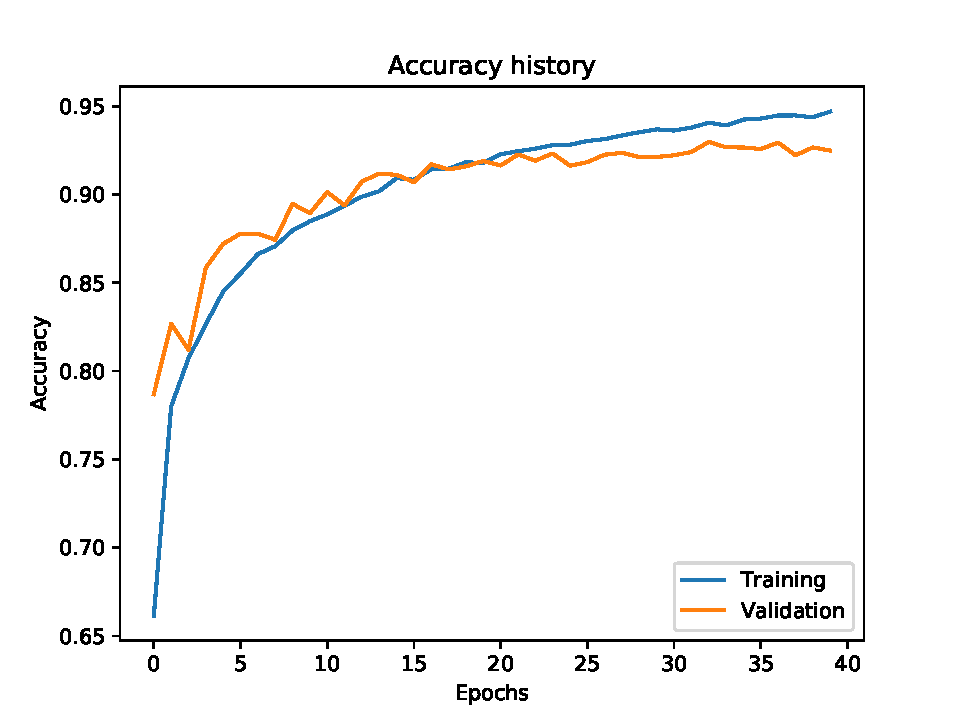
\includegraphics[width=.45\linewidth]{fig/accuracyhistoryequal.pdf}\label{fig:refstrukacc}}
  \end{subfigure}
 \begin{subfigure}[Verlustfunktion]{
 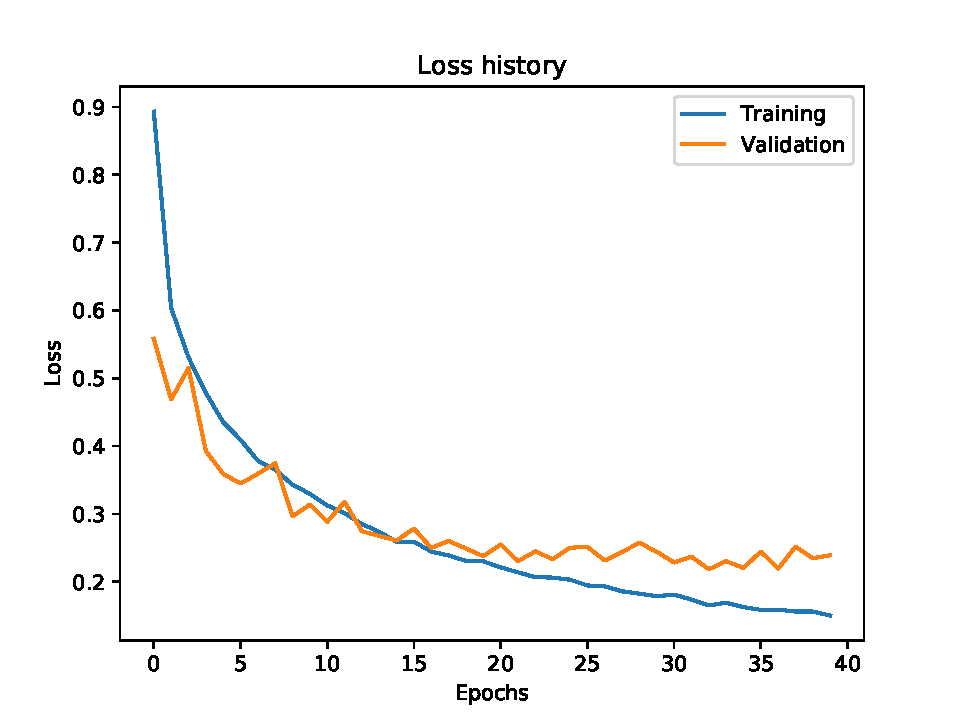
\includegraphics[width=.45\linewidth]{fig/losshistoryequal.pdf}\label{fig:refstrukloss}}
  \end{subfigure}
  \caption{Genauigkeit \ref{fig:refstrukacc} und Wert der Verlustfunktion \ref{fig:refstrukloss} nach jeder Epoche des Trainings bei Propagation des Trainings- und Validierungsdatensatzes durch das CNN mit der Referenzstruktur. }
  \label{fig:refstruk}
\end{figure}
\setcounter{subfigure}{0}
Anhand Abbildung \ref{fig:refstrukacc} lässt sich erkennen, dass die Referenzstruktur bereits gute Ergebnisse liefert, da eine Genauigkeit auf dem Validierungsdatensatz von über $90\,\%$ erzielt wird. Da sich weder die Genauigkeiten noch die Werte der Verlustfunktion auf dem Validierungsdatensatz stark von den entsprechenden Werten auf dem Trainingsdatensatz unterscheiden, liegt nur geringes Übertraining vor, wodurch auf weitere Optimierungen des CNN in Bezug auf die Verminderung des Übertrainings beispielsweise durch das Einfügen von zusätzlichen Dropout Lagen oder Regularisierung, verzichtet wird. \\
Als Maß für den Lernerfolg des CNN dient zudem die Verwirrungsmatrix, welche die prozentuale Verteilung der Aufnahmen einer Klasse auf die durch das CNN vorhergesagten Klassenzugehörigkeit angibt. Das bedeutet demnach, dass sich die Zeilen der Matrix zu $100\,\%$ addieren und die Matrix im Idealfall nur diagonale Einträge hat. Für die Referenzstruktur ist die Verwirrungsmatrix in \ref{fig:confmatun} dargestellt und es lässt sich eine diagonal dominante Struktur feststellen. Es lässt sich jedoch auch erkennen, dass die Aufnahmen der Klasse DRUSEN nur zu $64\,\%$ richtig werden. Wird anstelle der oben definierten Genauigkeit, die Genauigkeit des Netzes durch den Mittelwert der Prozentwerte der diagonalen Elemente angegeben, so ergibt sich eine Genauigkeit von $86\,\%$. Da es gewünscht ist, dass für jede Klasse die höchstmögliche Genauigkeit erreicht, wird diese Genauigkeit im Folgenden als Maß für den Lernerfolg verwendet und als Gesamtgenauigkeit bezeichnet. \\ 
\begin{figure}[!t]
 \centering
  \begin{subfigure}[Ungewichteter Datensatz]{
 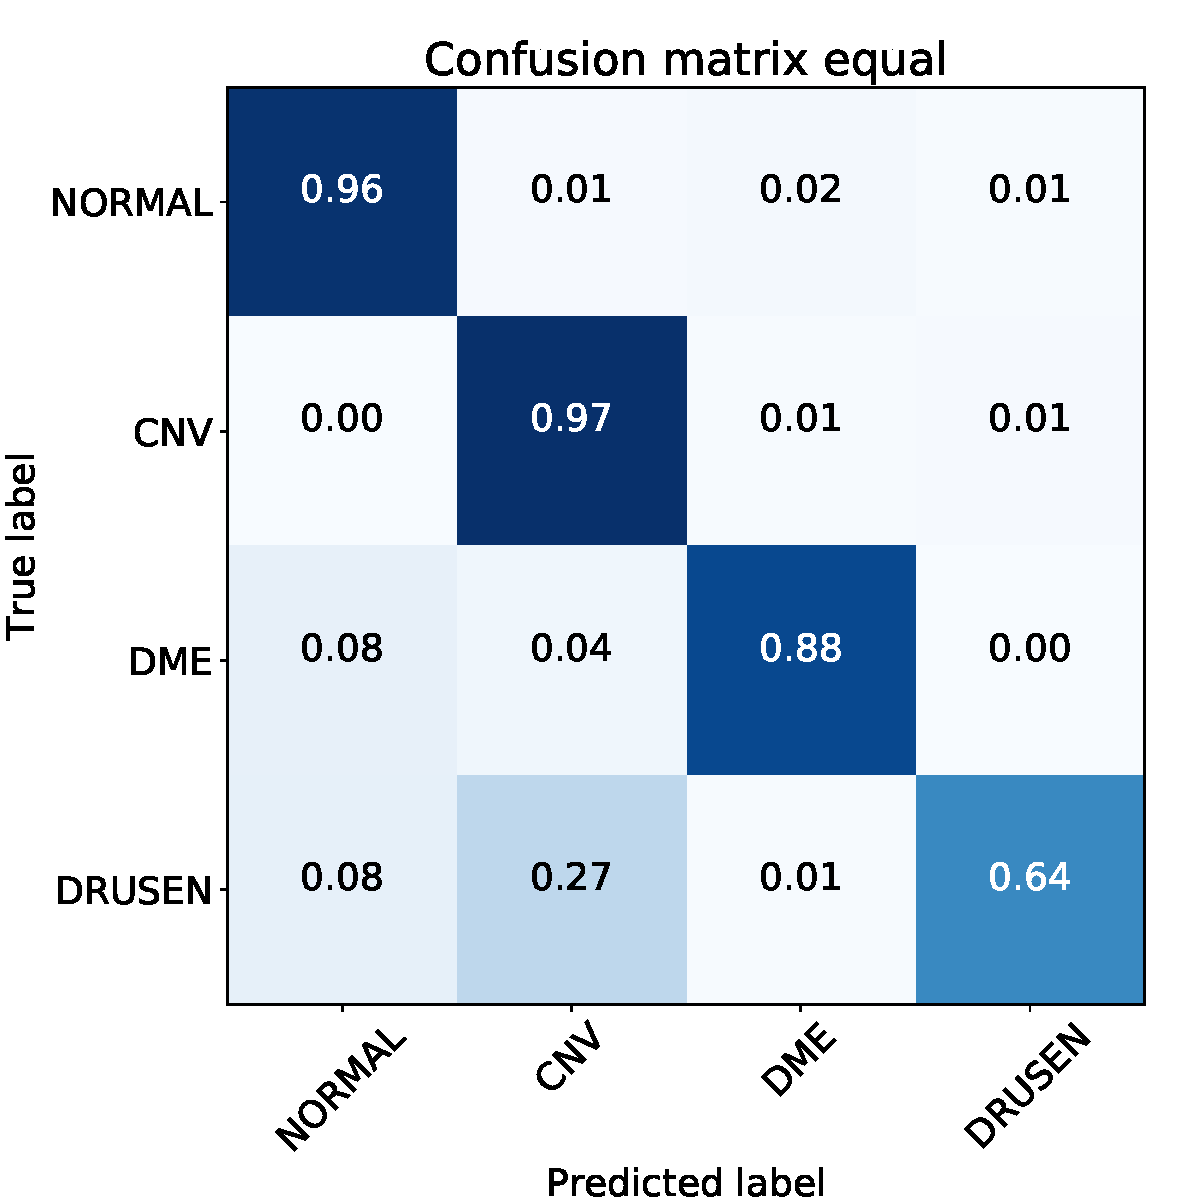
\includegraphics[width=.35\linewidth]{fig/confusionmatrixequal.pdf}\label{fig:confmatun}}
  \end{subfigure}
 \begin{subfigure}[Gewichteter Datensatz]{
 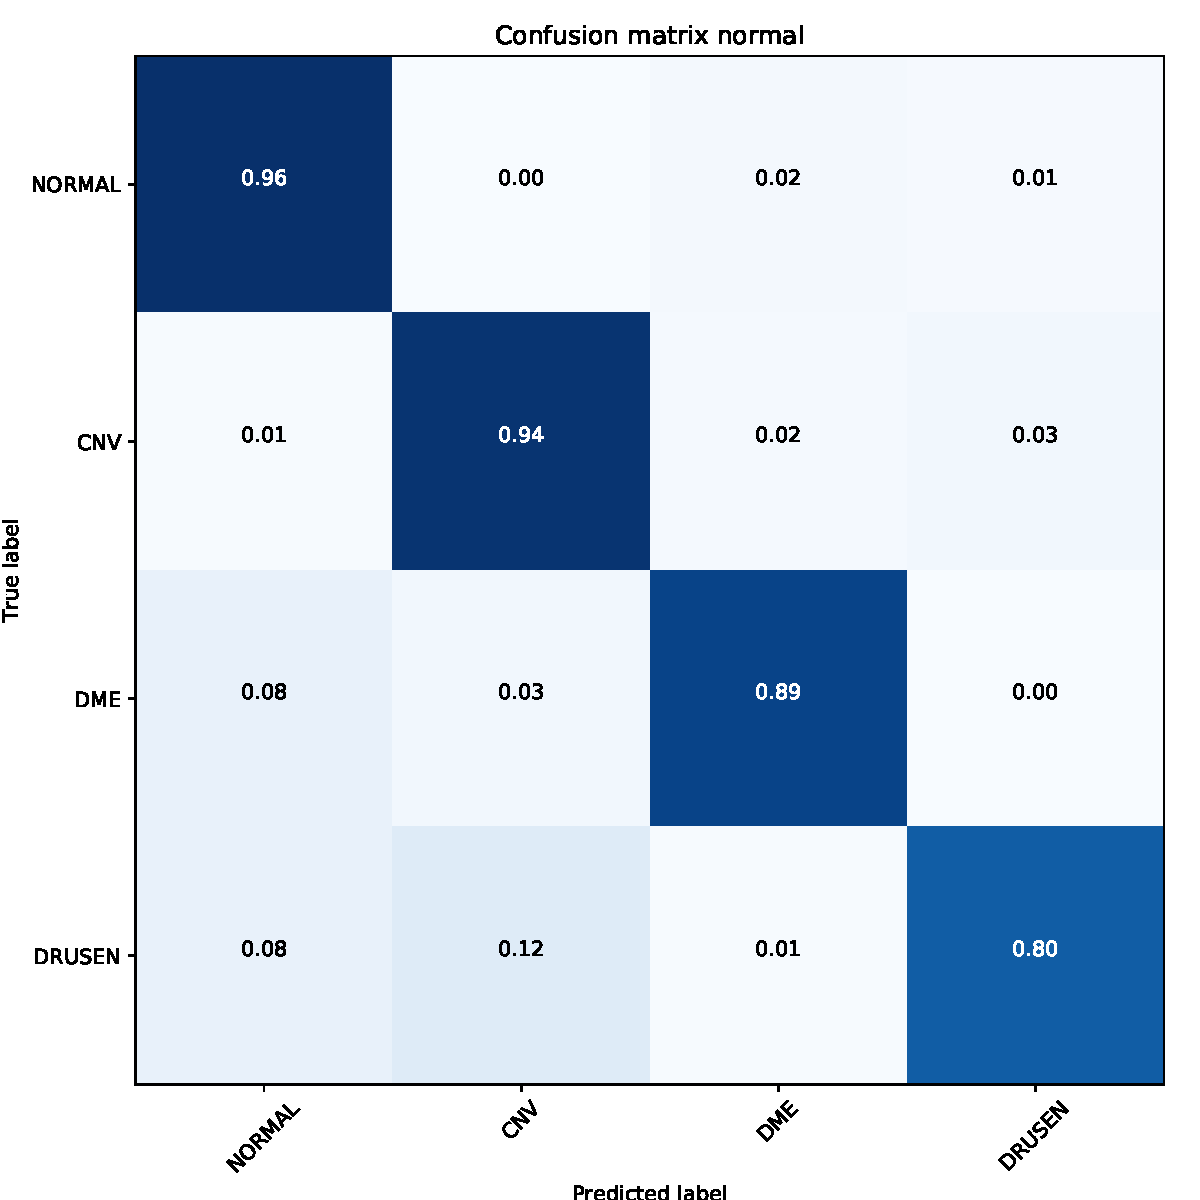
\includegraphics[width=.35\linewidth]{fig/confusionmatrixnormal.pdf}\label{fig:confmatweight}}
  \end{subfigure}
  \caption{Verwirrungsmatrizen nach dem Training ohne Gewichtung des Datensatzes in Abbildung \ref{fig:confmatun} und mit verwendeter Gewichtung in Abbildung \ref{fig:confmatweight}.}
  \label{fig:confmat}
\end{figure}
\setcounter{subfigure}{0} 
Wie sich in Tabelle \ref{tab:datacomp} erkennen lässt, sind die Klassen im Datensatz unterschiedlich stark repräsentiert. Die Klassen, die durch die Referenzstruktur am schlechtesten klassifiziert werden, sind die Klassen DME und DRUSEN, die am schwächsten im Datensatz vertreten sind. Um dies im Training zu berücksichtigen, wird jeder Aufnahme innerhalb des Datensatzes ein Gewicht zugeordnet, sodass sich die Gewichte der Aufnahmen innerhalb einer Klasse zu 1 addieren, und das Gewicht in der Verlustfunktion berücksichtigt. Für die Referenzstruktur ergibt dies die in Abbildung \ref{fig:confmatweight} dargestellte Verwirrungsmatrix. Die Gesamtgenauigkeit steigt hier auf $90\,\%$ und die Klasse DRUSEN wird deutlich besser klassifiziert und erreicht eine Gesamtgenauigkeit von $80\,\%$, wobei die anderen Klassen weiterhin sehr gut klassifiziert werden. Daher werden im Folgenden stets diese Gewichte im Training berücksichtigt.  \\ 
\begin{figure}[!t]
 \centering
  \begin{subfigure}[relu als Aktivierungsfunktion]{
 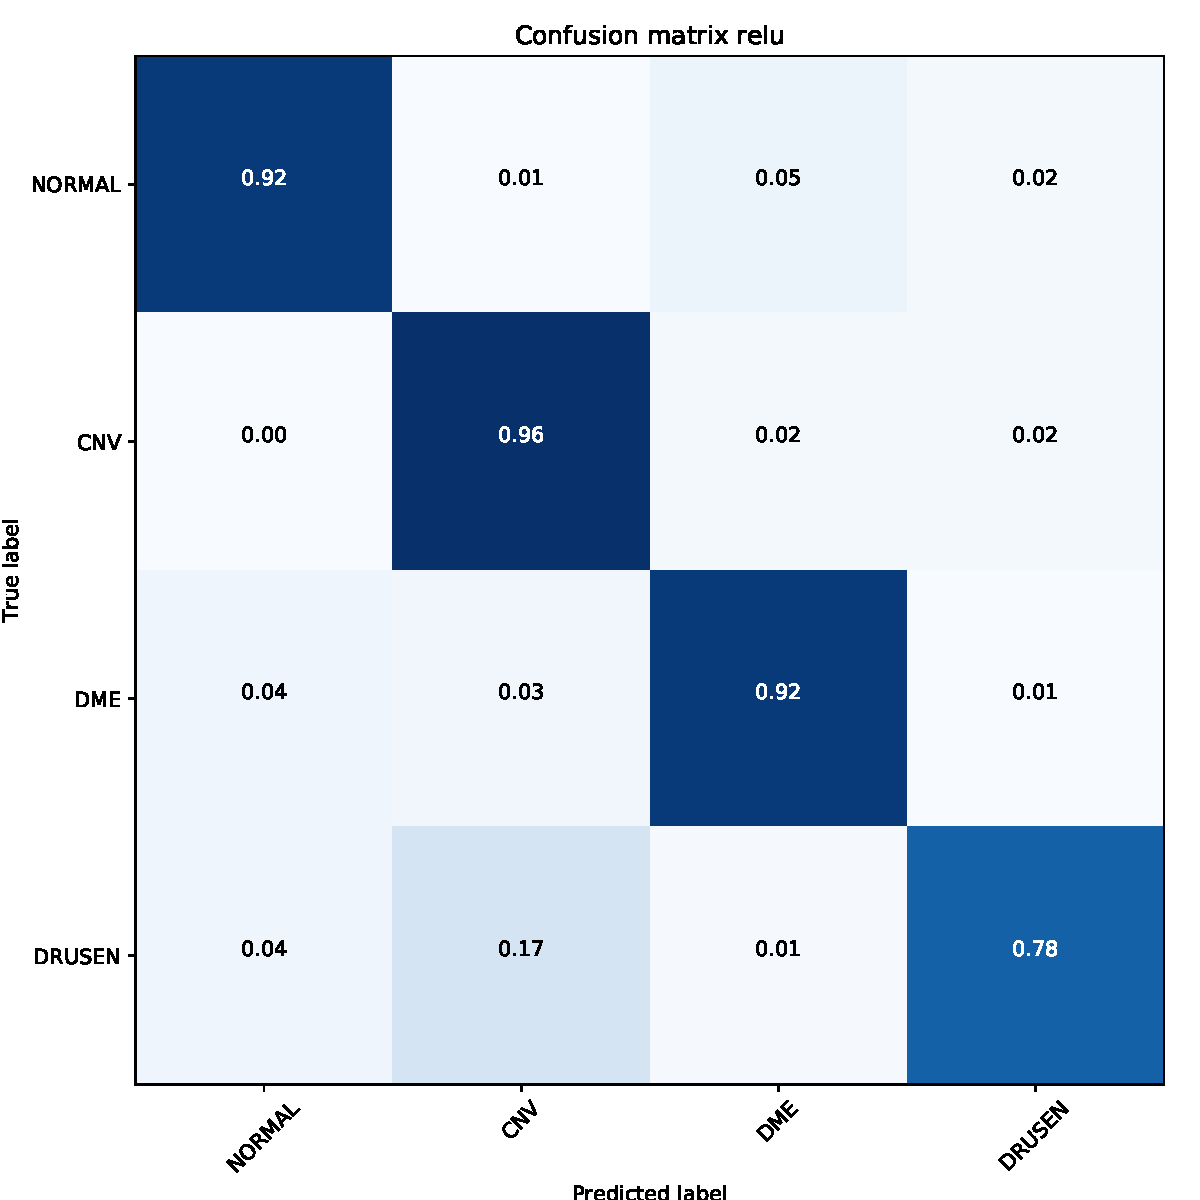
\includegraphics[width=.35\linewidth]{fig/confusionmatrixrelu.pdf}\label{fig:confmatrelu}}
  \end{subfigure}
 \begin{subfigure}[Veränderte Struktur des CNN]{
 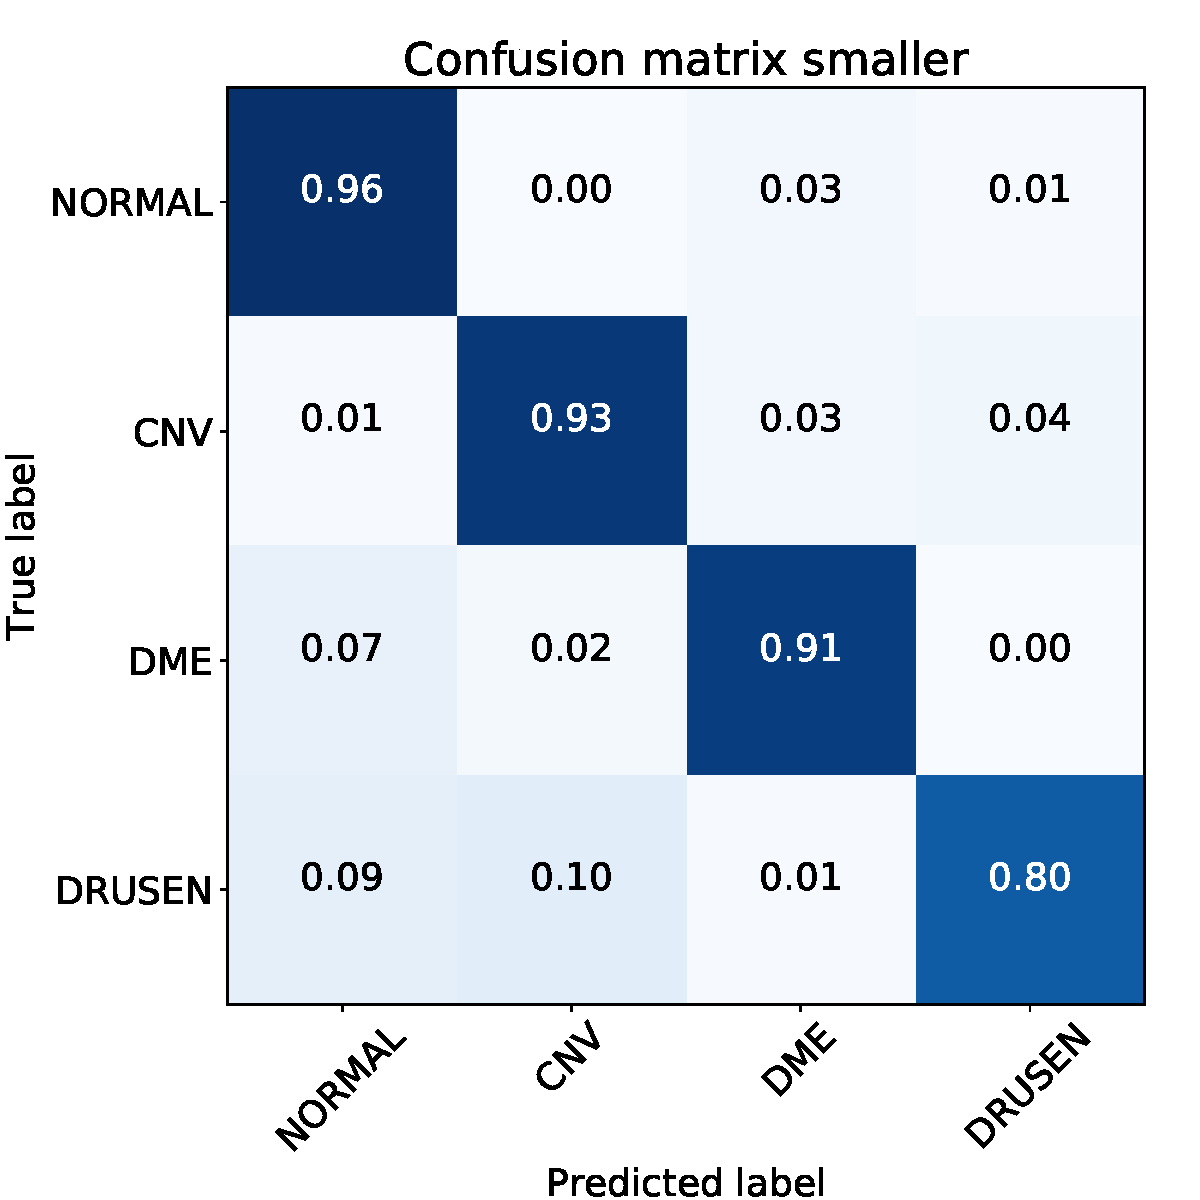
\includegraphics[width=.35\linewidth]{fig/confusionmatrixsmaller.pdf}\label{fig:confmatsmaller}}
  \end{subfigure}
  \caption{Verwirrungsmatrix bei Verwendung des gewichteten Datensatzes des CNN mit der Referenzstruktur mit relu als Aktivierungsfunktion der versteckten Lagen \ref{fig:confmatrelu} und veränderter Struktur der dichten Lagen \ref{fig:confmatsmaller}.}
  \label{fig:confmatrelusmall}
\end{figure}
\setcounter{subfigure}{0}
\begin{figure}[!b]
 \centering
   \begin{subfigure}[Genauigkeit]{
 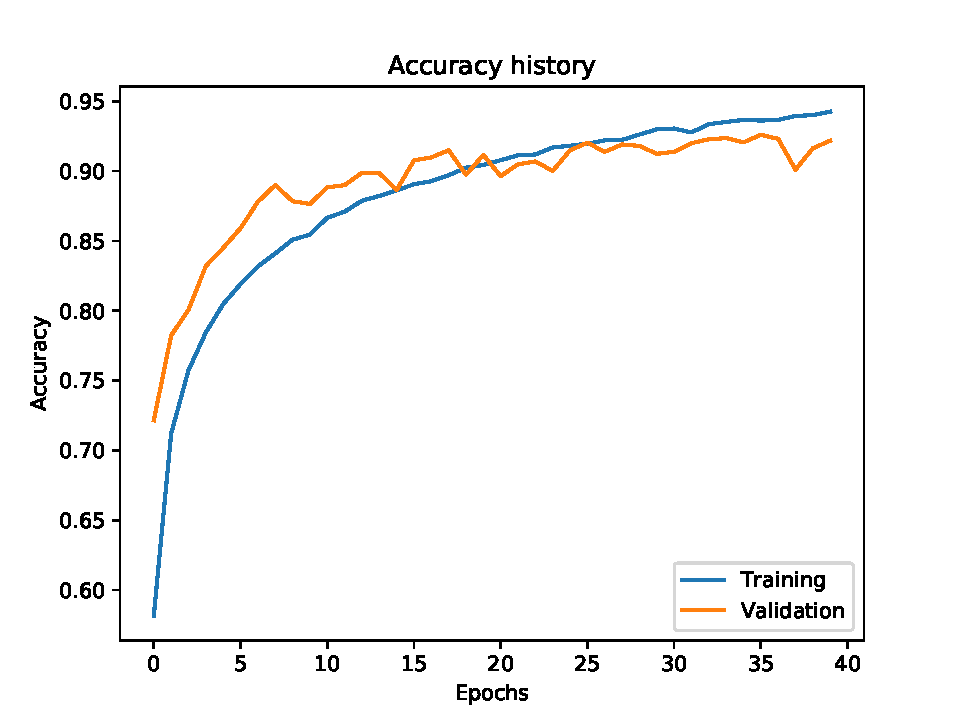
\includegraphics[width=.45\linewidth]{fig/accuracyhistorysmaller.pdf} \label{fig:accsmaller}}
  \end{subfigure}
 \begin{subfigure}[Verlustfunktion]{
 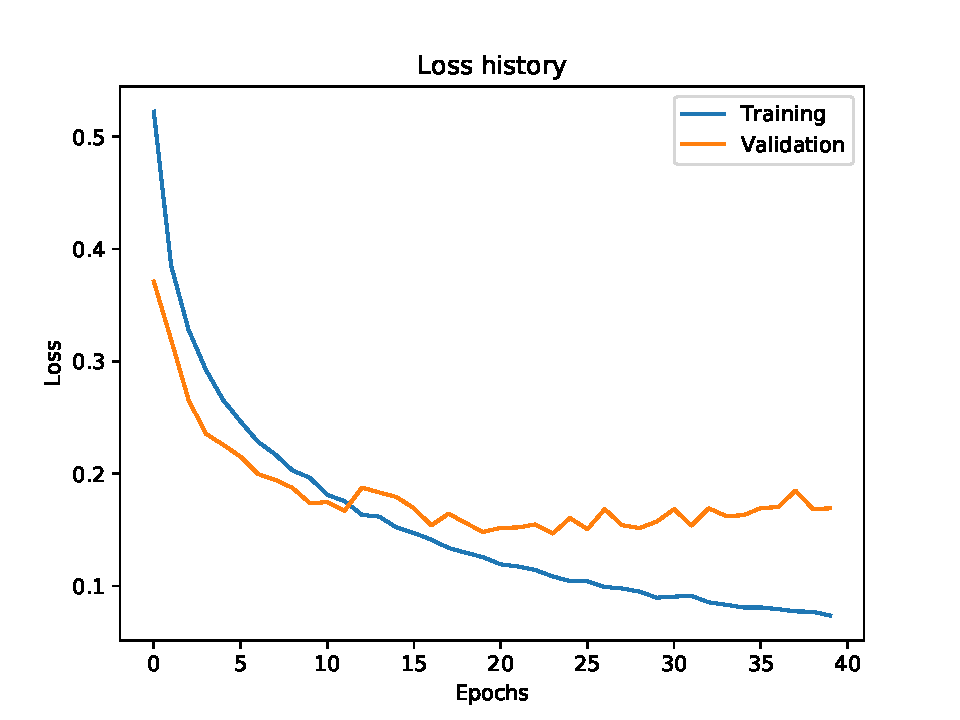
\includegraphics[width=.45\linewidth]{fig/losshistorysmaller.pdf}\label{fig:losssmaller}}
  \end{subfigure}
  \caption{Genauigkeit \ref{fig:accsmaller} und Wert der Verlustfunktion \ref{fig:losssmaller} nach jeder Epoche des Trainings bei Propagation des Trainingsdatensatzes und Validierungsdatensatzes durch das CNN mit der angepassten Struktur der dichten Lagen.}
  \label{fig:smallerperf}
\end{figure}
\setcounter{subfigure}{0} 
Die weiterführende Optimierung der Netzstruktur gestaltet sich als sehr zeitaufwendig, da das Training der Referenzstruktur bereits $17$ Stunden dauert. Daher werden im Folgenden zwei Optimierungsansätze diskutiert, die im Rahmen der Projektarbeit durchgeführt werden. Zunächst wird getestet, welche Auswirkung die Änderung der Aktivierungsfunktion der versteckten Lagen auf den Lernerfolg des CNN haben. In Abbildung \ref{fig:confmatrelu} ist die resultierende Verwirrungsmatrix dargestellt, wenn relu (rectified linear unit) anstelle von elu verwendet wird. Die Gesamtgenauigkeit ist mit $89\,\%$ etwas geringer, sodass keine Verbesserung erzielt werden kann.  \\
\begin{figure}[!b]
 \centering
  \begin{subfigure}[NORMAL]{
 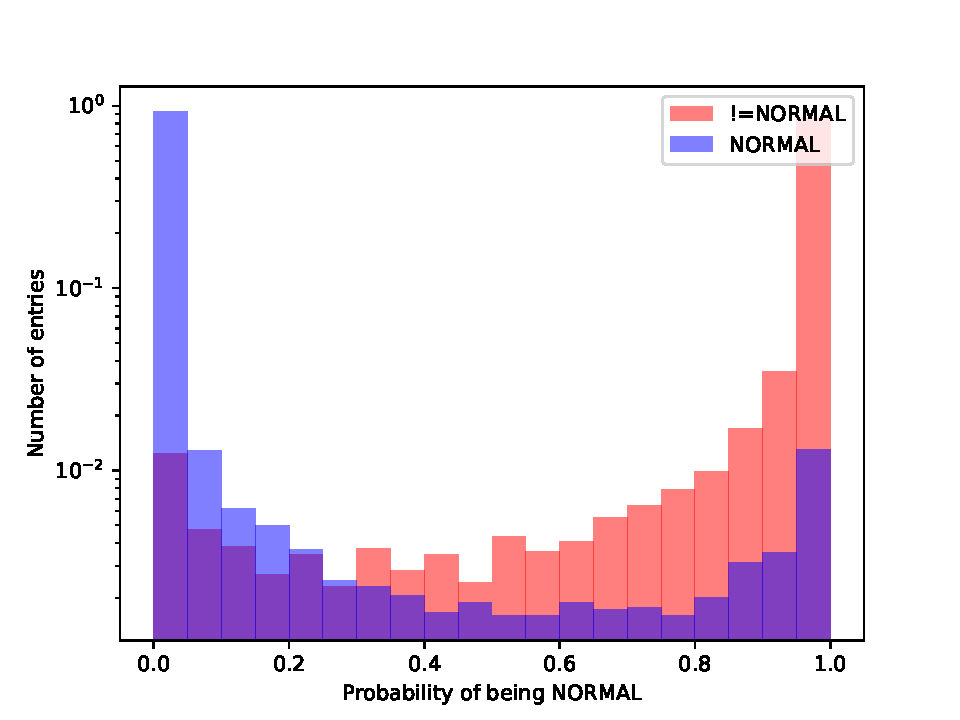
\includegraphics[width=.44\linewidth]{fig/NORMALornotlogsmaller.pdf} \label{fig:probnorm}}
  \end{subfigure}
 \begin{subfigure}[CNV]{
 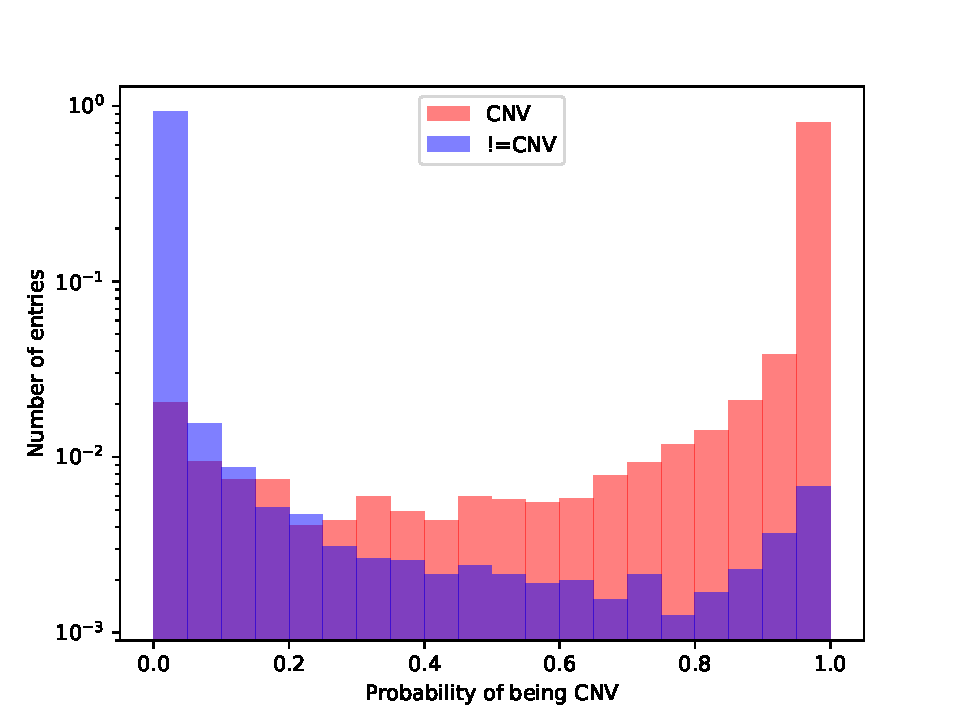
\includegraphics[width=.44\linewidth]{fig/CNVornotlogsmaller.pdf}\label{fig:probcnv}}
  \end{subfigure} \\
  \begin{subfigure}[DME]{
 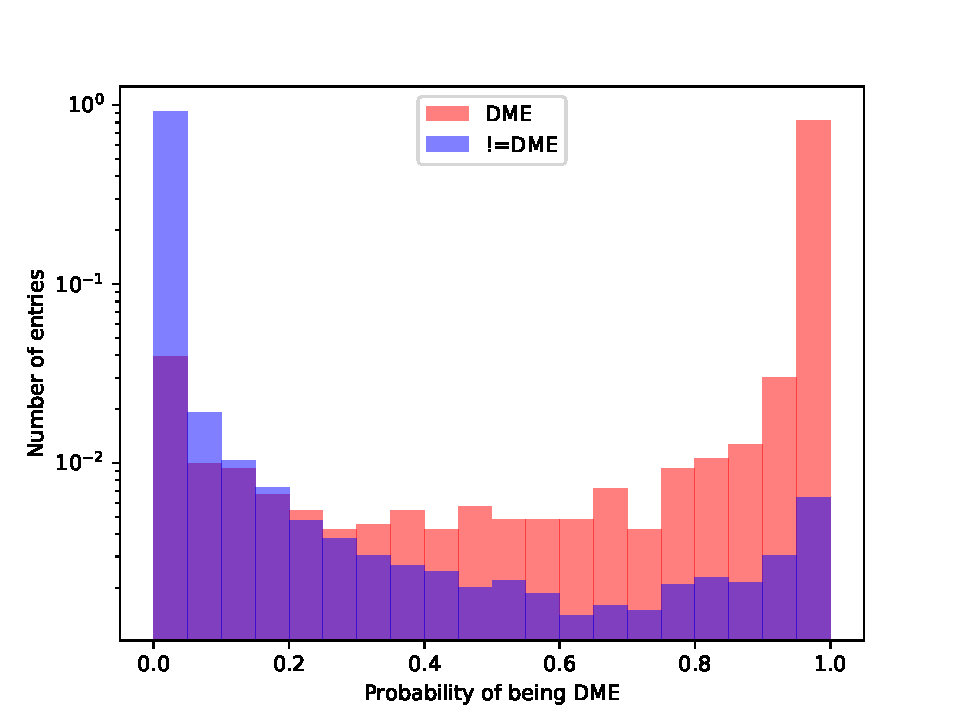
\includegraphics[width=.44\linewidth]{fig/DMEornotlogsmaller.pdf}\label{fig:probdme}}
  \end{subfigure}
 \begin{subfigure}[DRUSEN]{
 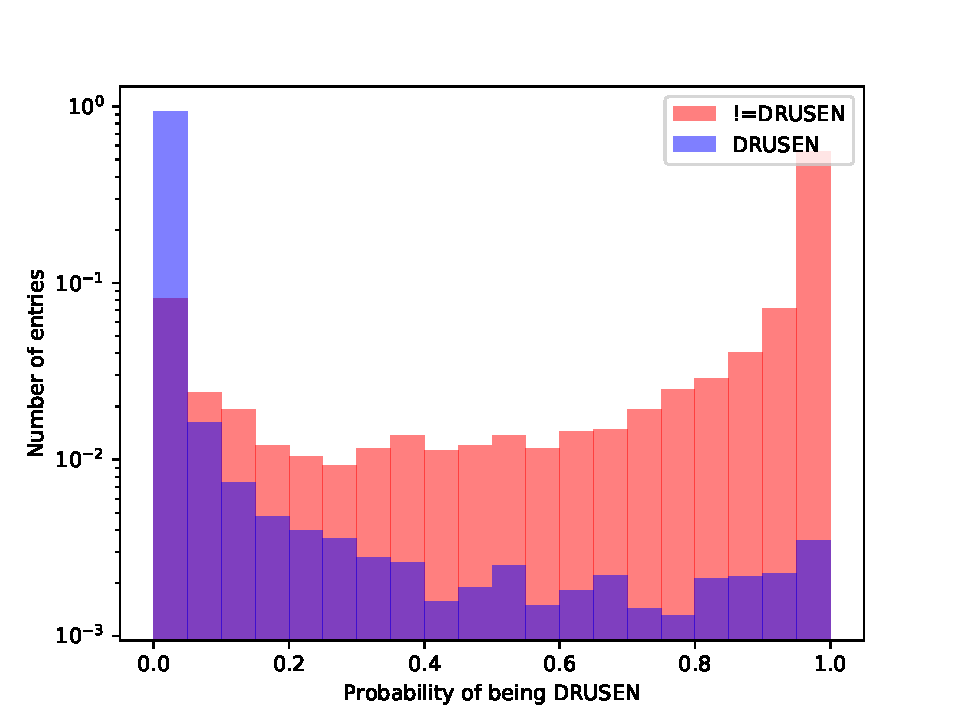
\includegraphics[width=.44\linewidth]{fig/DRUSENornotlogsmaller.pdf}\label{fig:probdrusen}}
  \end{subfigure}
  \caption{Verteilung der von dem CNN vorhergesagten Wahrscheinlichkeiten für die Aufnahmen innerhalb einer Klasse X und für die Aufnahmen, die nicht dieser Klasse angehören (!=X), der Klasse X anzugehören. Die Abbildungen \ref{fig:probnorm}, \ref{fig:probcnv}, \ref{fig:probdme} und \ref{fig:probdrusen} zeigen dies für die Klassen NORMAL, CNV, DME respektive DRUSEN. }
  \label{fig:probCNN}
\end{figure}
\setcounter{subfigure}{0} 
Zudem wird festgestellt, dass die erste dichte Lage nach der Flatten Lage enorm viele Parameter aufweist, sodass die Größe der dichten Lagen vor der Flatten Lage angepasst werden. Die Lage mit 1000 Neuronen wird auf 256 Neuronen, die Lage mit 256 Neuronen auf 128 Neuronen reduziert, wodurch sich zudem die Trainingsdauer stark vermindert. Die resultierenden Genauigkeitswerte und Werte der Verlustfunktion nach jeder Epoche und die Verwirrungsmatrix sind in den Abbildungen \ref{fig:accsmaller}, \ref{fig:losssmaller} respektive \ref{fig:confmatsmaller} dargestellt. Es lässt sich erkennen, dass sich die Genauigkeit leicht verbessert und $90\,\%$ beträgt. Somit wird diese Struktur als finale Struktur in dieser Projektarbeit verwendet. \\
Die Werte der Neuronen der Ausgangslage lassen sich als Wahrscheinlichkeiten für die Zugehörigkeit einer Aufnahmen zu einer Klasse interpretieren. Abbildung \ref{fig:probCNN} zeigt die Verteilungen der Wahrscheinlichkeitswerte für die Aufnahmen innerhalb einer Klasse X und für die Aufnahmen außerhalb einer Klasse X (!=X) der Klasse X anzugehören. Dies bedeutet anschaulich, dass im Idealfall die roten Verteilungen in Abbildung \ref{fig:probCNN} nur bei 1 Aufnahmen aufweisen, wohingegen die blauen Verteilungen nur bei 0 Aufnahmen aufweisen. Demnach liegt für alle Verteilungen eine sehr gute Diskriminierung von nicht der Klasse zugehörigen Aufnahmen vor. Jedoch zeigt Abbildung \label{fig:probdrusen}, dass für die Klasse DRUSEN die Wahrscheinlichkeitsverteilung der zu DRUSEN zugehörigen Aufnahmen im Vergleich zu den Abbildungen \ref{fig:probnorm}-\ref{fig:probdme} einen kleineren Ausschlag bei dem Wert 1 und eine deutlich höhere Flanke zu kleinen Werten aufweist, wodurch hier eine deutlich schwächere Diskriminierung vorhanden ist.  
 


% \begin{itemize}
%  \item Eingangslage mit Eingangsdaten der Form $(400\times 400)$ 
%  \item Conv2D Lage mit 64 Faltungsmatrizen der Dimension $(4 \times 4)$ und Schrittweite $(2,\,2)$ $\Rightarrow$ $(199 \times 199 \times 64)$ Ausgangsstruktur
%  \item Pooling Lage mit $(3\times 3)$ Fenster $\Rightarrow$ $(66 \times 66 \times 64)$ Ausgangsstruktur
%  \item Conv2D Lage mit 32 Faltungsmatrizen der Dimension $(4 \times 4)$ und Schrittweite $(2,\,2)$ $\Rightarrow$ $(32 \times 32 \times 32)$ Ausgangsstruktur
%  \item Pooling Lage mit $(3\times 3)$ Fenster $\Rightarrow$ $(10 \times 10 \times 32)$ Ausgangsstruktur
%  \item Dropout der Größe 0.25
%  \item Dichte Lage mit 1000 Neuronen $\Rightarrow$ $(10 \times 10 \times 1000)$ Ausgangsstruktur
%  \item Dichte Lage mit 250 Neuronen $\Rightarrow$ $(10 \times 10 \times 250)$ Ausgangsstruktur
%  \item Flatten Lage mit 25000 Ausgangsneuronen
%  \item Dichte Lage mit 100 Ausgangsneuronen
%   \item Dropout der Größe 0.5
%  \item Dichte Lage mit 32 Ausgangsneuronen
%  \item Dichte Ausgangslage mit 4 Ausgangsneuronen
% \end{itemize}